\chapter{MEASUREMENTS OF THE VISCOSITY OF THE QUASI-LIQUID LAYER AT THE SURFACE OF ICE-I$_\mathrm{h}$}\label{chap:QLL}

\begin{flushright}
\textit{``In time and with water, everything changes.''} \\
-Leonardo da Vinci (1513) \\
\end{flushright}

In the hydrodynamic friction regime, there are three distinct
contributions to the overall observed friction; the solid-liquid
friction between the ice and quasi-liquid layer (QLL), the viscous
shearing of the QLL, and the solid-liquid friction between the QLL and
the slider.\cite{Kietzig2009,Kietzig2010} In Chapter
\ref{chap:Friction}, we presented facet-dependent friction
coefficients for the basal, prismatic, 14\degree~pyramidal, and
secondary prism ice-I$_\mathrm{h}$ / water interfaces. In this
chapter, we present an investigation of the temperature dependence of
the shear viscosity of the QLL at the basal and prismatic
ice-I$_\mathrm{h}$ / vapor interfaces.



\section{Computational Methods}

\begin{flushleft}
\textit{Ice Surfaces}
\end{flushleft}

TIP4P-Ice basal and prismatic ice-I$_\mathrm{h}$ primitive crystals
were constructed following the procedure described in Chapter
\ref{chap:Methods}. These primitive cells were then reoriented so that
the desired crystal face was exposed to the $y$ axis, then replicated
in the $x$ and $z$ dimensions to form large sheets. The sheets were
then replicated in $y$ until the basal crystal was 12 bilayers thick,
and the prismatic crystal was replicated to a width of approximately
equal to the basal crystal. Dimensions and number of molecules in each
system are found in Table \ref{tab:qll-method}.


\begin{table}[h]
\centering
\caption{SIZES OF THE VAPOR EXPOSED ICE-I$_\mathrm{h}$ / QUASI-LIQUID LAYER SIMULATIONS\label{tab:qll-method}}
\begin{tabular}{rcccc}
\hline
\hline
 Interface & $N_\mathrm{ice}$ & $L_x$ & $L_y$ & $L_z$ \\
\hline
Basal  $\{0001\}$                           & 46,080 & 185.24 & 44.04 & 186.06 \\
Prismatic  $\{10\bar{1}0\}$            & 55,000 & 192.47 & 49.14 & 181.61\\
\hline
\hline
\end{tabular}
\begin{flushleft}
Box dimensions are given in \AA.
\end{flushleft}
\end{table}


The $y$-dimension of the simulation box was then set to 300~\AA~ to
allow for a surface premelt to form, and replicas of each system were
equilibrated to four temperatures, 255, 260, 265, and 270~K at
1~atm. The resulting systems exposed two interfaces, one toward
positive $y$ and the other towards negative $y$. Equilibration was
conducted under a constant surface tension and temperature integrator,
allowing the $x$ and $z$ dimensions of the simulation cell to relax
and alleviate any crystal strain. Following this, the systems were
equilibrated under a constant volume and temperature integrator (NVT),
and lastly under a constant volume and energy integrator (NVE). During
these simulations, the width of the crystal (in the $y$-dimension) was
monitored to ensure no appreciable crystal melt or large scale
restructuring occurred. Once equilibration was complete, a 100 ps
production simulation was performed for each system, where the
positions and velocities were recored every 0.1 ps.



% In Chapter \ref{chap:Str}, we found the
% tetrahedrality at the Gibbs dividing surface for ice-I$_\mathrm{h}$ /
% water interfaces to be $q^{Gibbs} \sim$0.84. Here, we have used
% $q^{Gibbs}$ as the cutoff value between the QLL and the ice. All
% molecules with $q < q^{Gibbs}$ are denoted as QLL molecules, while
% those with $q > q^{Gibbs}$ are denoted to be ice. This cutoff
% coincides with a minimum in the tangential density profiles, as seen
% in the top and bottom panels of Figure \ref{fig:qll-rhoq}.


\begin{flushleft}
\textit{Supercooled Liquids}
\end{flushleft}
As a comparison to the structure and dynamics of the quasi-liquid
layer of ice, we have performed simulations of supercooled bulk liquid using the
TIP4P/Ice potential. A cubic box of 4,000 water molecules was
constructed and replicas were equilibrated to 255~K, 260~K, 265~K, and
270~K. System sizes and corresponding densities are presented in Table
\ref{tab:qll-liquid}. Once the liquid boxes were equilibrated, four
successive one nanosecond simulations were performed under an NVE
integrator. During these simulations, the positions and velocities
were stored every 100 fs.

\begin{table}[h] \centering \caption{SYSTEM SIZES AND DENSITIES OF THE SUPERCOOLED BULK LIQUID\label{tab:qll-liquid}}
\begin{tabular}{cccc}
\hline
\hline
 Temperature & $N_\mathrm{molecules}$ & $L_x, L_y, L_z$ & $\rho$\\
\hline
270 & 4,000 & 50.1512 & 0.9487 \\
265 & 4,000 & 50.1305 & 0.9499 \\
260 & 4,000 & 50.1821 & 0.9469 \\
255 & 4,000 & 50.2494 & 0.9437 \\
\hline
\hline
\end{tabular}
\begin{flushleft}
Temperatures, box dimensions, and densities are given in K, \AA~, and
$\mathrm{g}~\mathrm{cm}^{-3}$, respectively.
\end{flushleft}
\end{table}

\section{Characterization of the Quasi-Liquid Layer}
Formation of a quasi-liquid layer on the basal and prismatic surfaces
of ice-I$_\mathrm{h}$ was observed at all temperatures
investigated. Characterizing this surface premelt can be achieved by a
variety of order parameters. Here, we have chosen two structural
parameters, the local density and the local tetrahedral order
parameter described in Chapter \ref{chap:Str}. To compute profiles of
these measures, each of the systems investigated were divided into
small bins ($\delta y$) and an average of the order parameter was
computed for that bin. The resulting profiles for the basal and
prismatic systems at each temperature are presented in Figures
\ref{fig:basal_rhoq} and \ref{fig:prism_rhoq}.

\begin{figure*}
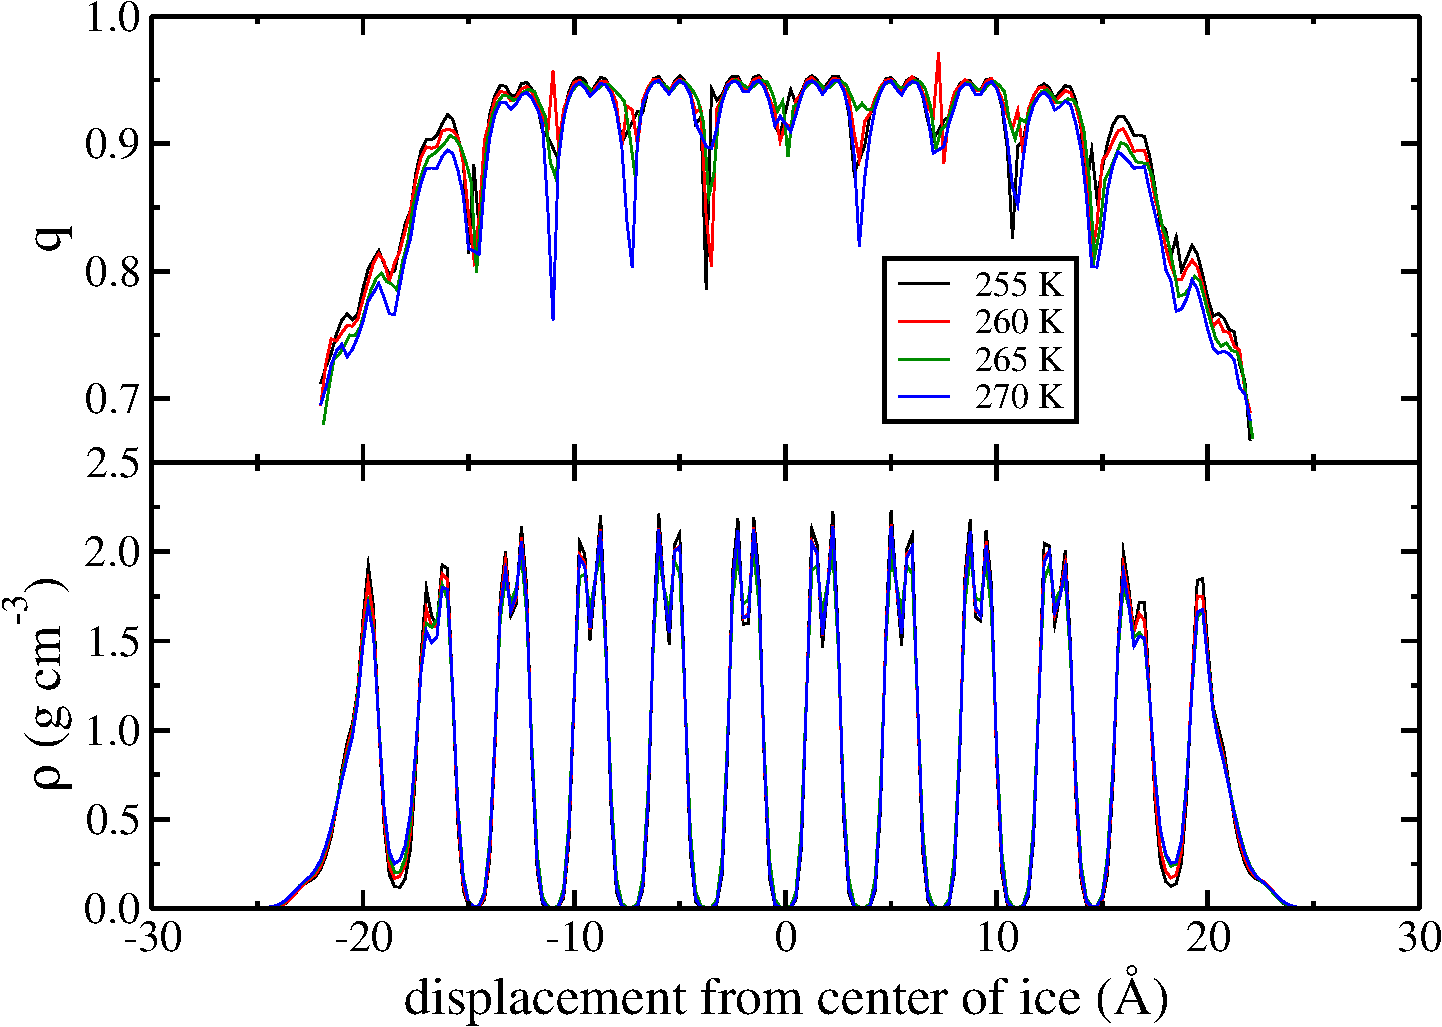
\includegraphics[width=\linewidth]{Figures/basal_rhoq}
\caption{\label{fig:basal_rhoq} The spatially resolved average density
  (lower) and local tetrahedral order parameter (upper) of the
  exposed basal ice-I$_\mathrm{h}$ crystal. Quasi-liquid layer
  formation is observed in the outermost water bilayers.}
\end{figure*}                


\begin{figure*}
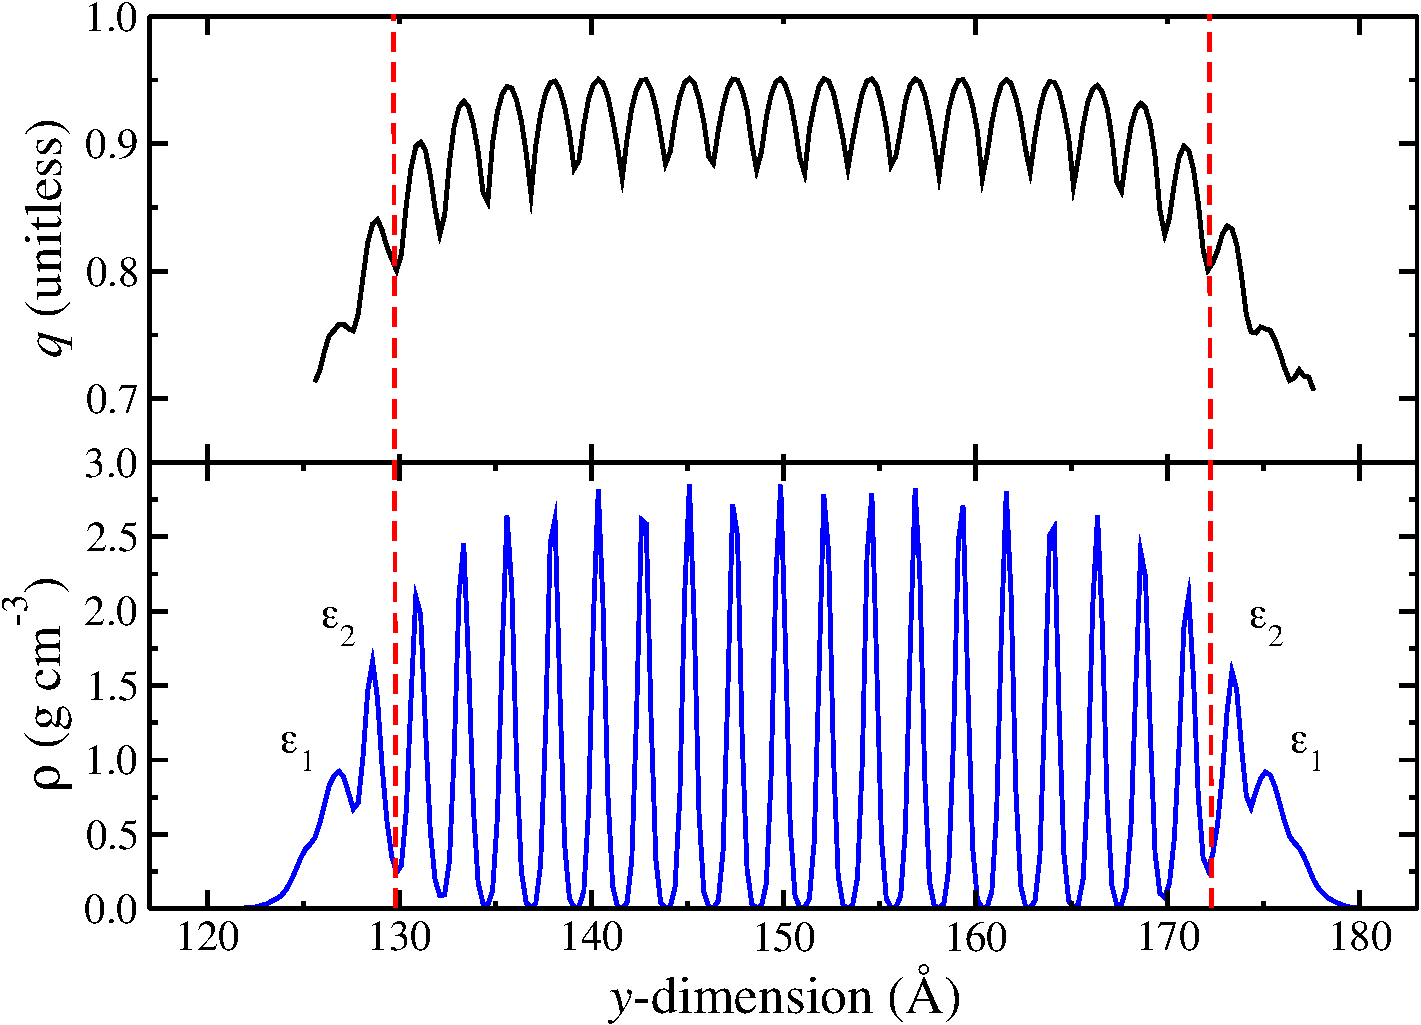
\includegraphics[width=\linewidth]{Figures/prism_rhoq}
\caption{\label{fig:prism_rhoq} Panel description matches that of
  Figure \ref{fig:basal_rhoq}, but for the exposed prismatic
  ice-I$_\mathrm{h}$ crystal. }
\end{figure*}                

In the lower panel of Figure \ref{fig:basal_rhoq}, the local density
for the basal systems shows a formation of a QLL at a displacement of
$~\sim\pm$ 21 \AA~ from the center of the ice. The peaks around these
displacements shows wetting of the underlying crystal. That is, the
density does not go to zero between the crystal and liquid planes. Interior to
this, the characteristic bilayer of ice is observed in the twin peaks
at each plane of ice. Note the outter peaks have lost this bilayer
distribution, further indicating its liquid-like character. Comparing
the density profiles for the four temperatures investigated, we
observe a greater extent of wetting of the underlying crystal for
warmer temperatures. Similarly, the height of the QLL peak decreases
with warmer temperature, indicating a more liquid-like environment.

In the bottom panel of Figure \ref{fig:prism_rhoq}, the
local density for the prismatic systems indicates a quasi-liquid layer
formation around $\sim\pm$ 24. While the basal QLL density was found
to be $\rho~ \sim$~1.5 - 2.0 $\mathrm{g}~\mathrm{cm}^{-3}$, we observe
densities closer to 1.0 $\mathrm{g}~\mathrm{cm}^{-3}$ at the prismatic
surface. Also, the prismatic QLL appears to more completely wet the underlying
ice crystal when compared with the basal surface premelt. The same
trend with increasing temperature is observed at the prismatic
surface; at warmer temperatures the QLL's density comes closer to
that of the bulk liquid. 

In the upper panels of the same figures are the local tetrahedral
order parameter profiles through the interface. For the basal
interface in Figure \ref{fig:basal_rhoq}, we see the characteristic
bilayer shapes in the tetrahedrality profile. Interior to the ice, we
observe $q$ values close to 0.95, indicating a very tetrahedral
environment. In the peak determined to be a QLL using density
measures, the parameter takes on values of 0.9 to 0.85. Beyond
displacements of $\pm$~22 \AA~ from the center of the ice lies the
vapor, and $q$ becomes small and noisy. The profile presented in
Figure \ref{fig:prism_rhoq} for the prismatic interface appears very
similar to that of the basal interface. It is interesting to note, that since
the tetrahedral order parameter depends on neighboring molecules, it
indicates that the crystal plane interior to the QLL layer determined
by the density also deviates from bulk-like environments. This stems
from the outer layer contributing less to its $q$ value. However,
this could indicate that this first interior layer should also be
denoted as a QLL, although perhaps more appropriately named a
quasi-solid layer (QSL).



\section{The Shear Viscosity of the Quasi-Liquid Layer}
According to kinetic theory, the diffusion constant, $D$, can be
related to the mobility ($\mu$) of a particle and the temperature,
$T$.
\begin{equation}
D = \mu k_B T
\end{equation}
The mobility is often described as the ratio of the particle's
terminal velocity $v_d$ to an applied force $F$. A specialized form of
this relation relates the diffusion constant to the shear viscosity
($\eta$) of the fluid.
\begin{equation}\label{eq:stokes-einst}
D = \frac{k_BT}{4\pi \eta r}
\end{equation}
This relation was first derived by Einstein to determine the diffusion
constant for a ``Stokes'' particle of radius $r$ undergoing Brownian
Motion.

In order to compute estimates of the shear viscosity, spatially
resolved diffusion constants were computed along the dimension normal
to the interface.
\begin{equation}\label{eq:yDiff}
D(y) = \frac{1}{6t} \langle | \mathbf{r}_i(t) - \mathbf{r}_i(0) |^2
\delta(y_i(0) - y)  \rangle 
\end{equation}
Equation \eqref{eq:yDiff} was computed in 1 \AA~. In the lower portion
of Figures \ref{fig:basal_DEta} and \ref{fig:prism_DEta} diffusion
profiles are shown for the basal and prismatic surfaces,
respectively. In the ice crystal, the diffusion coefficient is
numerically zero. At displacements of $\sim \pm$ 18 from the center of
the ice crystal, the diffusion coefficient becomes non-zero, and is
observed to rise parabolically through the QLL and into the vapor. For
both the basal and prismatic systems, there is a suggested temperature
dependence when observing the lower interface, however, resolution at
the upper interface prevents a definitive argument to be made.

\begin{figure*}
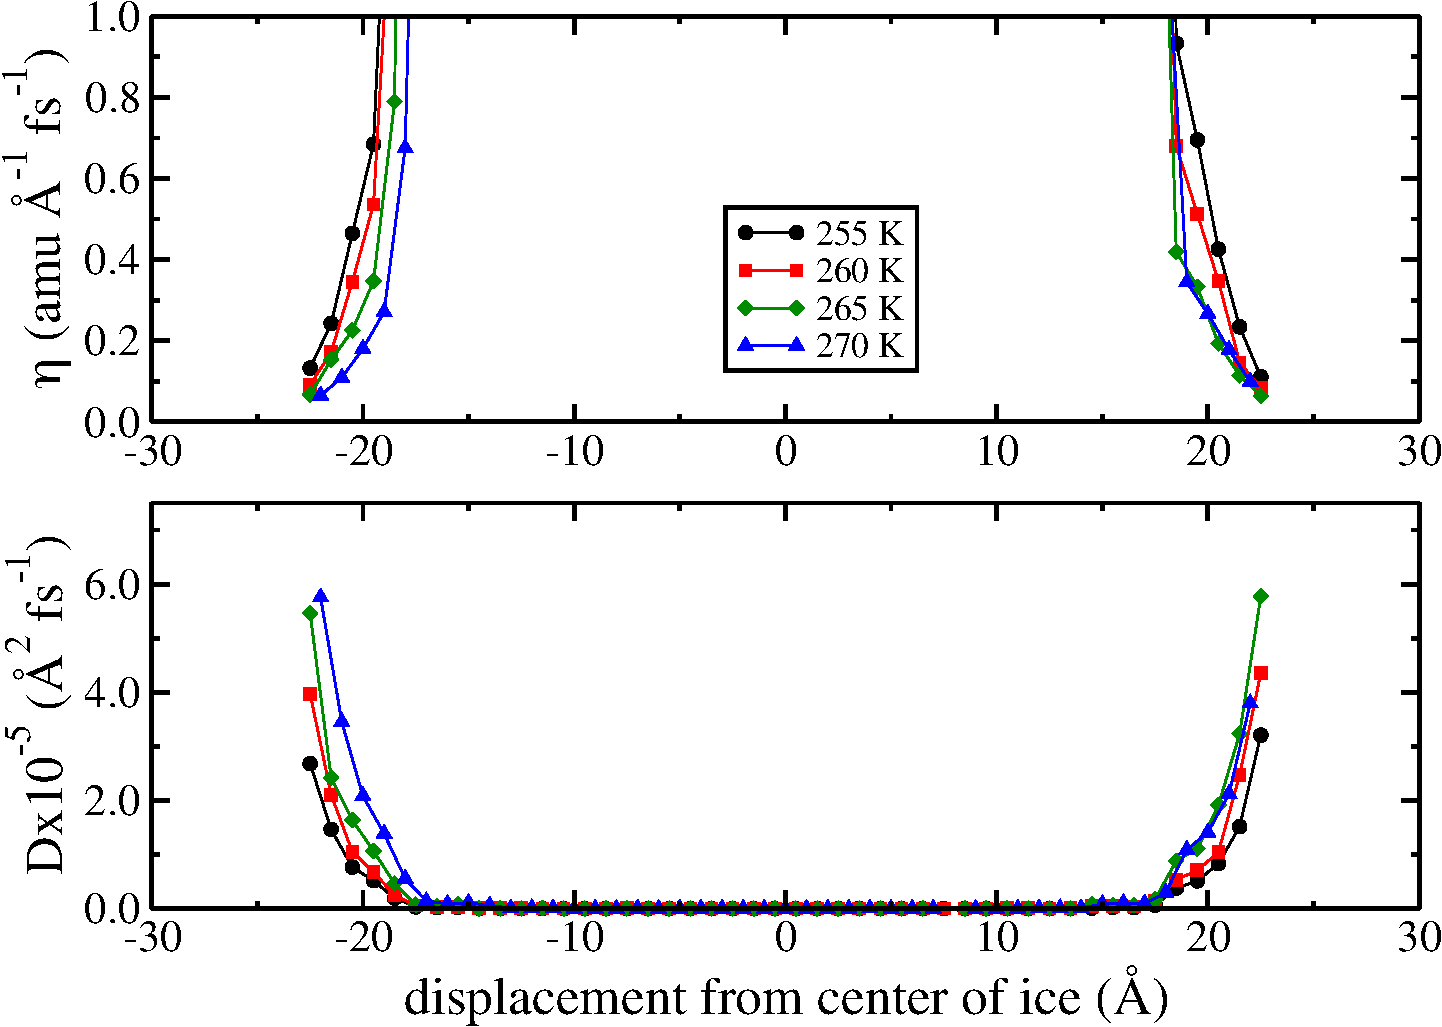
\includegraphics[width=\linewidth]{Figures/basal_2DEta}
\caption{\label{fig:basal_DEta} Lower: Spatially resolved diffusion
  coefficients for an exposed basal surface of an
  ice-I$_\mathrm{h}$ crystal. Upper: Spatially resolved shear viscosity
  at the same interface.}
\end{figure*}                

\begin{figure*}
\includegraphics[width=\linewidth]{Figures/prism_2DEta}
\caption{\label{fig:prism_DEta} Lower: Spatially resolved diffusion
  coefficients for an exposed prismatic surface of an
  ice-I$_\mathrm{h}$ crystal. Upper: Spatially resolved shear viscosity
  at the same interface.}
\end{figure*}                

From the diffusion coefficients, estimates of the shear viscosity
using Equation \eqref{eq:stokes-einst} is straightforward. These
results are shown in the top panels of Figures \ref{fig:basal_DEta}
and \ref{fig:prism_DEta}. In the vapor, we observe shear viscosities
close to zero.  $\eta$ increases through the QLLs, and rises
asymptomatically to infinity in the ice. Again, a slight
temperature dependence is suggested through the lower interface,
however, resolution of the upper interface prevents a conclusive
argument being made. 

We attempted to compute the shear viscosity of the quasi-liquid layers
in a second way. Using VSS-RNEMD \cite{Kuang2012}, a shear stress was
applied only to molecules in the QLLs. The VSS-RNEMD exchange regions
were defined to incorporate molecules from both the top and bottom
interfaces, and partitioning between the vapor, QLLs, and the ice
surfaces was performed using the local tetrahedral order parameter of
the water molecules. However, application of the VSS-RNEMD moves
resulted in non-linear behavior in the velocity distributions of the
QLLs. The surface premelts were found to couple more strongly with the
underlying ice than the neighboring QLL, resulting in dissipation of
the velocity ``kicks'' into the ice instead of in the surface
premelt. Due to this, we were unable to resolve shear viscosities
using the VSS-RNEMD method.



\section{Simulations of Supercooled Liquid}
Henson \textit{et al.} predicted that the QLL should behave as a
supercooled bulk liquid.\cite{Henson2005} Studying supercooled liquids
experimentally, however, can be quite challenging. Besides possibly
skewing results, contaminants can also act as nucleation sites for
crystal growth. Due to this, much of our insight on supercooled liquid
water comes from molecular simulations. Crystal growth is an extremely
slow process on the computational timescale, allowing for
investigations of bulk liquid in this temperature regime. 

\subsection{Structural Measures of Supercooled Water}

\begin{flushleft}
\textit{Pair Distribution Function}
\end{flushleft}

The pair distribution function, $\mathrm{g}(r)$, provides information
regarding the spatial distribution of molecules. Calculation of this
function was achieved by compiling the average number of molecules
found to be a distance $r$ to ($r + \delta r$) apart. The
pair density $\rho (r)$ of each of these small shells is normalized by
the system's bulk density and the shell volume.
\begin{equation}\label{eq:gofr}
\mathrm{g}(r) = \rho(r) / \rho^{bulk}
\end{equation}
Equation \eqref{eq:gofr} is a general relation which can be used for
pairs of atoms, molecules, or even assemblies. Here, we have have
computed $\mathrm{g}(r)$ for pairs of water molecules, as
seen in the lower panel of Figure \ref{fig:gofrQ}

\begin{figure*}
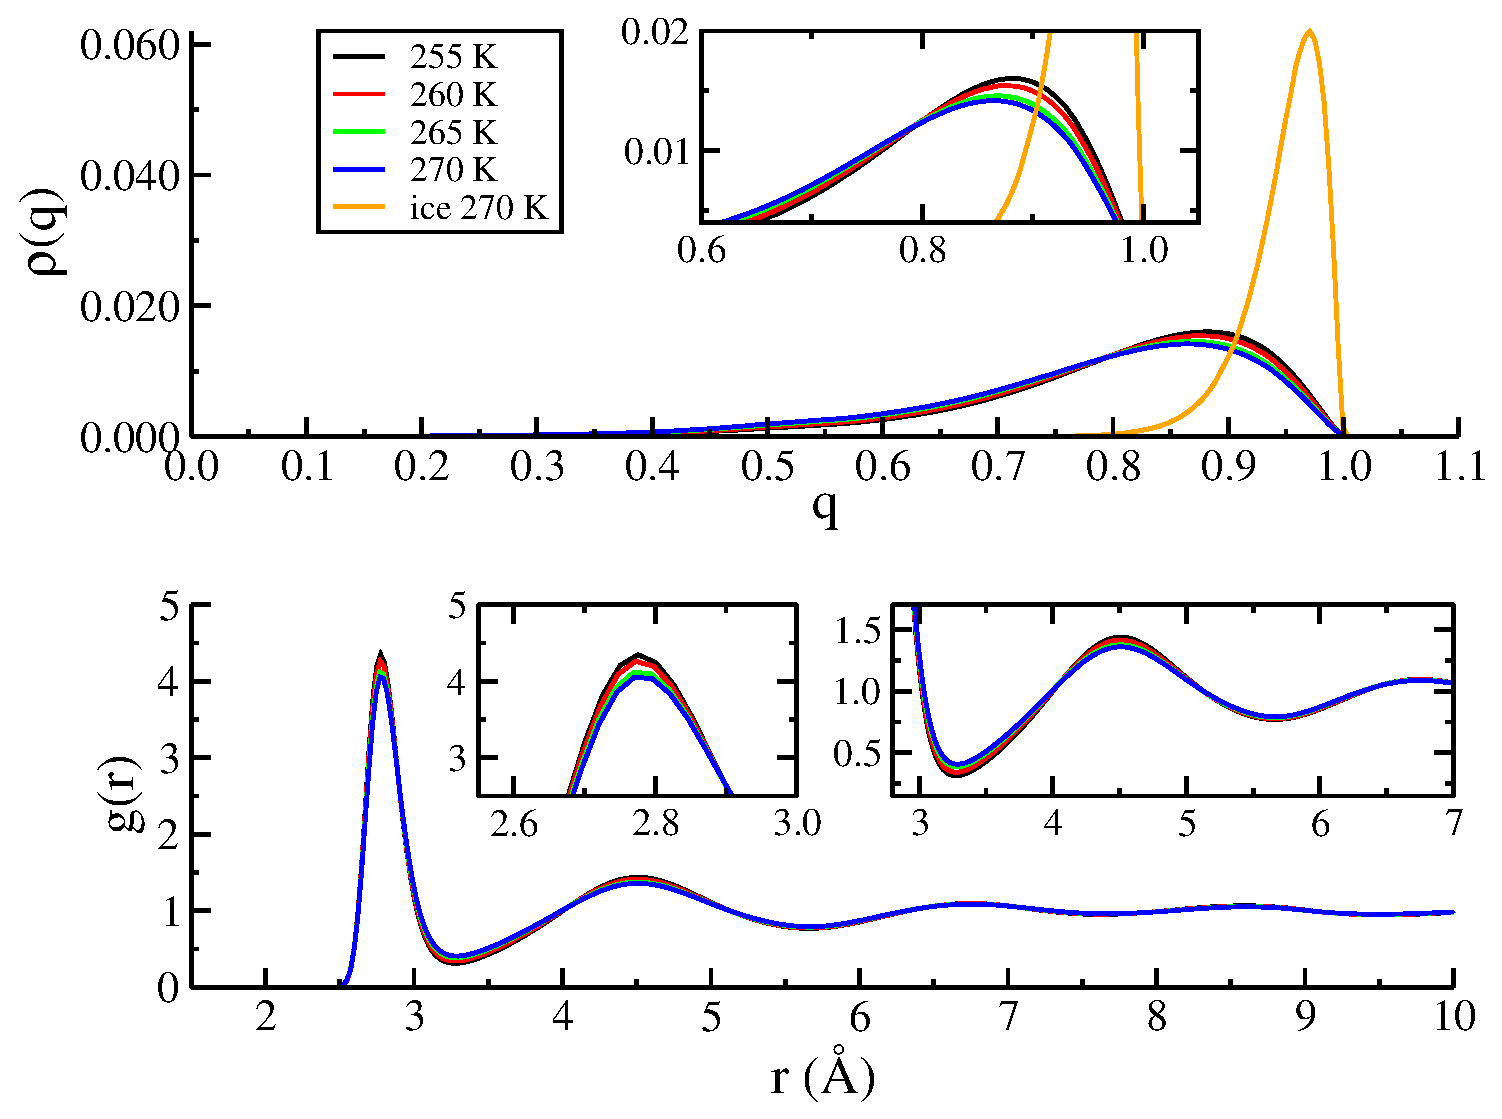
\includegraphics[width=\linewidth]{Figures/bulk_GofrQdens}
\caption{\label{fig:gofrQ} Pair distribution function
  $\mathrm{g}(r)$ and probability density distributions of
  the local tetrahedral order parameter $\rho (\mathrm{q})$ for
  supercooled liquid.}
\end{figure*}  

We observe no population of pairs of water molecules at small values
of $r$. This is due to the size of a water molecule, modeled
by the repulsive portion of the Lennard-Jones potential. The large
peak at $r~\sim$ 2.8 corresponds to the first solvation
shell around the water molecules. The dip immediately following this
peak indicates a region of low population, followed by a second
smaller peak. This second peak captures the second solvation shell of
water, which is more diffuse than the first. At larger values of
$r$ the function approaches unity, indicating at large
separations the liquid ordering reflects that of the bulk. 

The two insets are closer views of the first and second solvation
shells. We see for colder temperature, the liquid becomes slightly
more ordered, apparent from the increase in the first and second
solvation shells, as well as the decrease in the population between
the two shells. In order to quantify this ordering, it is
common to integrate $\mathrm{g}(r)$ to determine the
coordination number $n_c$.
\begin{equation}\label{eq:nofr}
n_c = 4 \pi \rho^{bulk} \int_0^{r_m} g(r)r^2dr
\end{equation}


\begin{table}[h] \centering \caption{LOCATION AND INTEGRATION OF THE
    RADIAL DISTRIBUTION FUNCTION AT THE FIRST SOLVATION SHELLS AND
    FRACTIONAL DENSITIES OF NUMBER OF HYDROGEN BONDS FORMED FOR
    SUPERCOOLED LIQUID\label{tab:gofr}}
\begin{tabular}{ccccccc}
  \hline
  \hline
  Temperature & $r_m$ & $n_c$ & $\rho_\mathrm{HB}(2)$ & $\rho_\mathrm{HB}(3)$ & $\rho_\mathrm{HB}(4)$ & $\rho_\mathrm{HB}(5)$ \\
  \hline
  270 & 3.297 &4.1523(3) & 0.01645(3) & 0.1531(9) & 0.7771(3) & 0.05231(1)\\
  265 & 3.271 & 4.1056(7) & 0.01447(57) & 0.1432(4) & 0.7907(8) & 0.0507(2)\\
  260 & 3.299 & 4.060(1) & 0.01126(6) & 0.1246(3) & 0.8172(4) & 0.0462(2)\\
  255 & 3.253 & 4.06024(6)  & 0.0096(1) & 0.1138(4) & 0.8330(9) &
                                                                  0.0431(4) \\
  \hline
  \hline
\end{tabular}
\begin{flushleft}
Temperatures are reported in K. Uncertainties are given in parentheses.
\end{flushleft}
\end{table}

We find that the location of the minimum following the first peak
$r_m$ in $\mathrm{g}(r)$ is at slightly larger values of $r$ with
increasing temperature. Taking this as the limit of integration, the
coordination number for the first solvation shell, $n_c$ was computed
(see Table \ref{tab:gofr}). Similarly, it is observed to increase with
increasing temperature. Since the supercooled liquid's density
increases with increasing temperature, we should expect a larger
coordination number with increasing temperature in this regime.

\begin{flushleft}
\textit{Density of Hydrogen Bonds}
\end{flushleft}

It is well known that water forms four hydrogen bonds in hexagonal
ice. In the liquid, water often adapts configurations which results in
a smaller number of hydrogen bonds. As an additional probe of the
supercooled liquid structure, we have computed the average fractional
populations of hydrogen bond participation ($\rho_\mathrm{HB}$) at
each of the four temperatures. To do so, we have used the hydrogen
bonding criteria of Luzar and Chandler, which requires the
oxygen-oxygen distance to be less than 3.4~\AA~, and the
oxygen-hydrogen-oxygen angle to be less than
30\degree~.\cite{Luzar1996} This criteria has been shown to give good
agreement with energetic definitions of hydrogen bonds, as the
geometric and energetic definitions are intimately coupled. The
resulting fractional participation statistics can be seen in Table
\ref{tab:gofr}.


% \begin{table}[h] \centering \caption{FRACTIONAL DENSITIES OF NUMBER OF
%     HYDROGEN BONDS FORMED FOR SUPERCOOLED LIQUID\label{tab:bulk_HB}}
% \begin{tabular}{ccccc}
% \hline
% \hline
%  Temperature & $\rho_\mathrm{HB}(2)$ & $\rho_\mathrm{HB}(3)$ & $\rho_\mathrm{HB}(4)$ & $\rho_\mathrm{HB}(5)$  \\
% \hline
% 270 & 0.01645(3) & 0.1531(9) & 0.7771(3) & 0.05231(1)\\
% 265 & 0.01447(57) & 0.1432(4) & 0.7907(8) & 0.0507(2)\\
% 260 & 0.01126(6) & 0.1246(3) & 0.8172(4) & 0.0462(2)  \\
% 255 & 0.0096(1) & 0.1138(4) & 0.8330(9) & 0.0431(4) \\
% \hline
% \hline
% \end{tabular}
% \begin{flushleft}
% Temperatures are reported in K. Uncertainties are given in parentheses.
% \end{flushleft}
% \end{table}

Here, we observe a clear temperature dependence on the fractional
populations of of hydrogen bonds participation formed in the
liquid. At colder temperatures, we find a larger fraction of the
population form four hydrogen bonds. However, at warmer temperatures,
the reduction in population of four hydrogen bonded molecules results
in larger densities of two, three, and five hydrogen bonded molecules.



\begin{flushleft}
\textit{Density of Tetrahedral Ordering}
\end{flushleft}

While the pair distribution function provides information about
the spatial separation of molecules, it fails to discriminate any
orientational ordering which may be present in the liquid. In order to
query this orientational ordering, the density of local tetrahedral
order parameters ($\rho (q)$) observed during the simulation was
computed (see Figure \ref{fig:gofrQ}). This was accomplished by
computing $q$ for every molecule each configuration, and determining
the fractional number of molecules which adopted this configuration.

In Figure \ref{fig:gofrQ}, we see a noticeable trend in $\rho (q)$
with increasing temperature. The $q$-value of the peak in the density
distribution decreases with increasing temperature. This indicates
that for warmer simulation temperatures, the tetrahedral ordering of
the liquid decreases. All four liquid simulations give a much broader
distribution than observed for a commensurate ice-I$_\mathrm{h}$
crystal at 270 K.





\subsection{Dynamic Measures of Supercooled Water}
At colder temperatures, we should expect the dynamics of water to be
slower simply due to lower kinetic energy. However, at colder
temperatures, water molecules may adapt structures which further hinder
dynamics. Since the density of tetrahedrality indicated an
orientational ordering in the liquid which was sensitive to
temperature, we may expect to observe temperature dependent dynamics
as well. Here, we have investigated both \textit{translational} and
\textit{orientational} measures of dynamics.

\begin{flushleft}
\textit{Diffusion in the Supercooled Liquid}
\end{flushleft}

Diffusion coefficients for water molecules in ice are approximately
zero, as the small amount of diffusion that is observed is highly
dependent on the presence of lattice defects. In contrast, diffusion
of water molecules in supercooled liquid is observed well below the
freezing point.\cite{Debenedetti2003} Pruppacher has measured the
diffusion of supercooled liquid down to -25\degree~C using a tritium
tracer.\cite{Pruppacher1972} In order to compare with the diffusion of
the quasi-liquid layers, we have computed three dimensional diffusion
coefficients for each of the bulk liquid simulations. Mean squared
displacements were computed for each of the supercooled liquid systems
(see lower panel of Figure \ref{fig:bulkD}), and the non-spatially
resolved version of Equation \eqref{eq:yDiff} was used to compute
average diffusion coefficients (see upper panel of the same figure).

\begin{figure*}
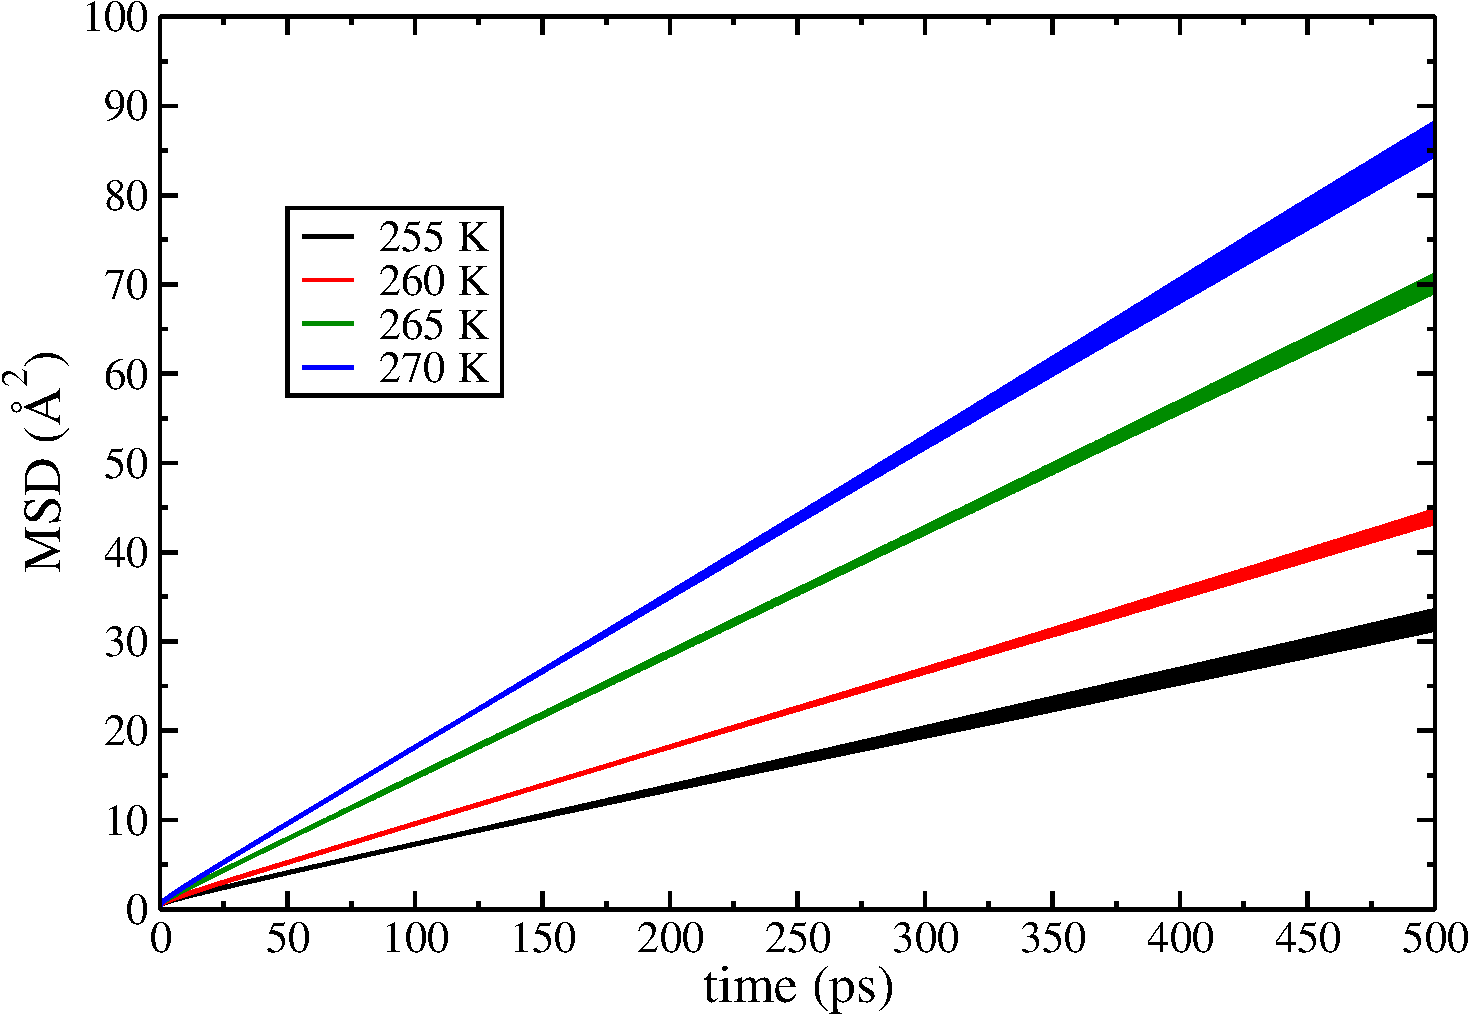
\includegraphics[width=\linewidth]{Figures/bulkD}
\caption{\label{fig:bulkD} Lower panel: mean squared displacements
  (MSD) for supercooled liquid water. Upper panel: three dimensional
  diffusion constants computed from the MSD data in the lower panel. }
\end{figure*}    
 
We estimate diffusion coefficients of
$\mathrm{D}~\sim~ 1.0 \times 10^{-5}
(\mathrm{\AA}^{2}~\mathrm{fs}^{-1})$ to
$\mathrm{D}~\sim~ 3.0 \times 10^{-5}
(\mathrm{\AA}^{2}~\mathrm{fs}^{-1})$ for the range of temperatures
investigated. % The data are fit well with a linear regression giving a
% rate of change between the data of
% $0.1254 \times 10^{-5}~\mathrm{D}/\mathrm{K}$.


\begin{flushleft}
\textit{Orientational Decorrelation}
\end{flushleft}

Orientational time correlation functions provide information on the
decorrelation of molecular environments. As we observed in Chapter
\ref{chap:Dyn}, decorrelation times in ice go asymptotically to
infinity, while in liquid, values in the ps to ns range are more
common. In Chapter \ref{chap:Dyn} we computed a spatially resolved
version of the orientational time correlation function to probe how
the dynamics of molecules changed approaching the ice-I$_\mathrm{h}$ /
water interface. Here, all of the water molecules should behave
identically over a long time average as there are no interfaces present.
\begin{equation}\label{C(t)}
  C_{2}(t)=\langle P_{2}(\mathbf{u}_i(0)\cdot \mathbf{u}_i(t))\rangle,
\end{equation}
Again, $P_2$ is the second-order Legendre polynomial, 
$\mathbf{u}_i$ is the molecular unit vector that bisects the HOH angle
of molecule $i$, and the angle brackets denotes an average over all
molecules and time origins. Computed C$_2$(t) is shown in the lower
panel of Figure \ref{fig:jump_lcorr}.

There are three modes available for decorrelation of $C_2(t)$. Fitting
computed $C_2(t)$ by a triexponential decay which captures the
characteristic times for these modes can provide insight on the
temperature dependence of the reorientation of supercooled liquid
water. The three time constants: $\tau_\mathrm{short}$, measuring the
librational motion of the water molecules, $\tau_\mathrm{middle}$,
measuring the timescale for the large angle jumps during the breaking
and making of hydrogen bonds, and $\tau_\mathrm{long}$, corresponding
to the translational motion of the water molecules, can be obtained
by\cite{Louden2013a}
\begin{equation}
  C_{2}(t) = a~e^{-t/\tau_\mathrm{short}} + b~e^{-t/\tau_\mathrm{middle}} + 
  (1-a-b)~e^{-t/\tau_\mathrm{long}}.
\label{eq:c2}
\end{equation}
Here, the coefficients $a$, $b$, and $(1-a-b)$ give the fractional
amount of the total decay due to that particular mode. Averages of the
decay constants and their coefficients are reported in Table
\ref{tab:supOrient}.


\begin{table}[h] \centering \caption{OREINTATIONAL DECAY TIMES AND
    THEIR FRACTIONAL CONTRIBUTIONS FOR SUPERCOOLED WATER\label{tab:supOrient}}
\begin{tabular}{ccccccc}
\hline
\hline
 Temperature & $a$ & $\tau_\mathrm{short}$& $b$ &
                                                  $\tau_\mathrm{middle}$
  & $(1-a-b)$ & $\tau_\mathrm{long}$\\
\hline
270 &0.2235(3) &85.1(3) & 0.165(2) & 3.75(5) & 0.611(2) & 26.1(2)\\
265 &0.2191(4) &86.0(2) & 0.174(4) & 4.8(1) & 0.607(5) & 34(1)\\
260 &0.2117(3) &87.5(2) & 0.190(6) & 7.7(3) & 0.599(6) & 59(1)\\
255 &0.2060(5) &87.2(4) & 0.183(7) & 9.6(5) & 0.611(8) & 81(2)\\
\hline
\hline
\end{tabular}
\begin{flushleft}
Temperatures are given in K, $\tau_{short}$ is reported in fs, while $\tau_{middle}$ and
$\tau_{long}$ are given in ps. Uncertainties are given in parentheses.
\end{flushleft}
\end{table}

We observe a very clear temperature dependence in
$\tau_\mathrm{short}$, $\tau_\mathrm{middle}$, and
$\tau_\mathrm{long}$; for increasing temperatures, the decay time
decreases. We find the fast librational motion decay time to be
between 85 fs and 87 fs, while the slower hydrogen bond dynamics and
frame reorientation characteristic times of 4-10 ps, and 26-80 ps
respectively.  Interestingly, the fractional contribution of each of
the modes is observed to be invariant with temperature. The
librational mode and the hydrogen bond breaking and making events each
account for about 20$\%$ of the total decay, with the remaining 60$\%$
of the decay given by frame reorientation.


\begin{figure*}
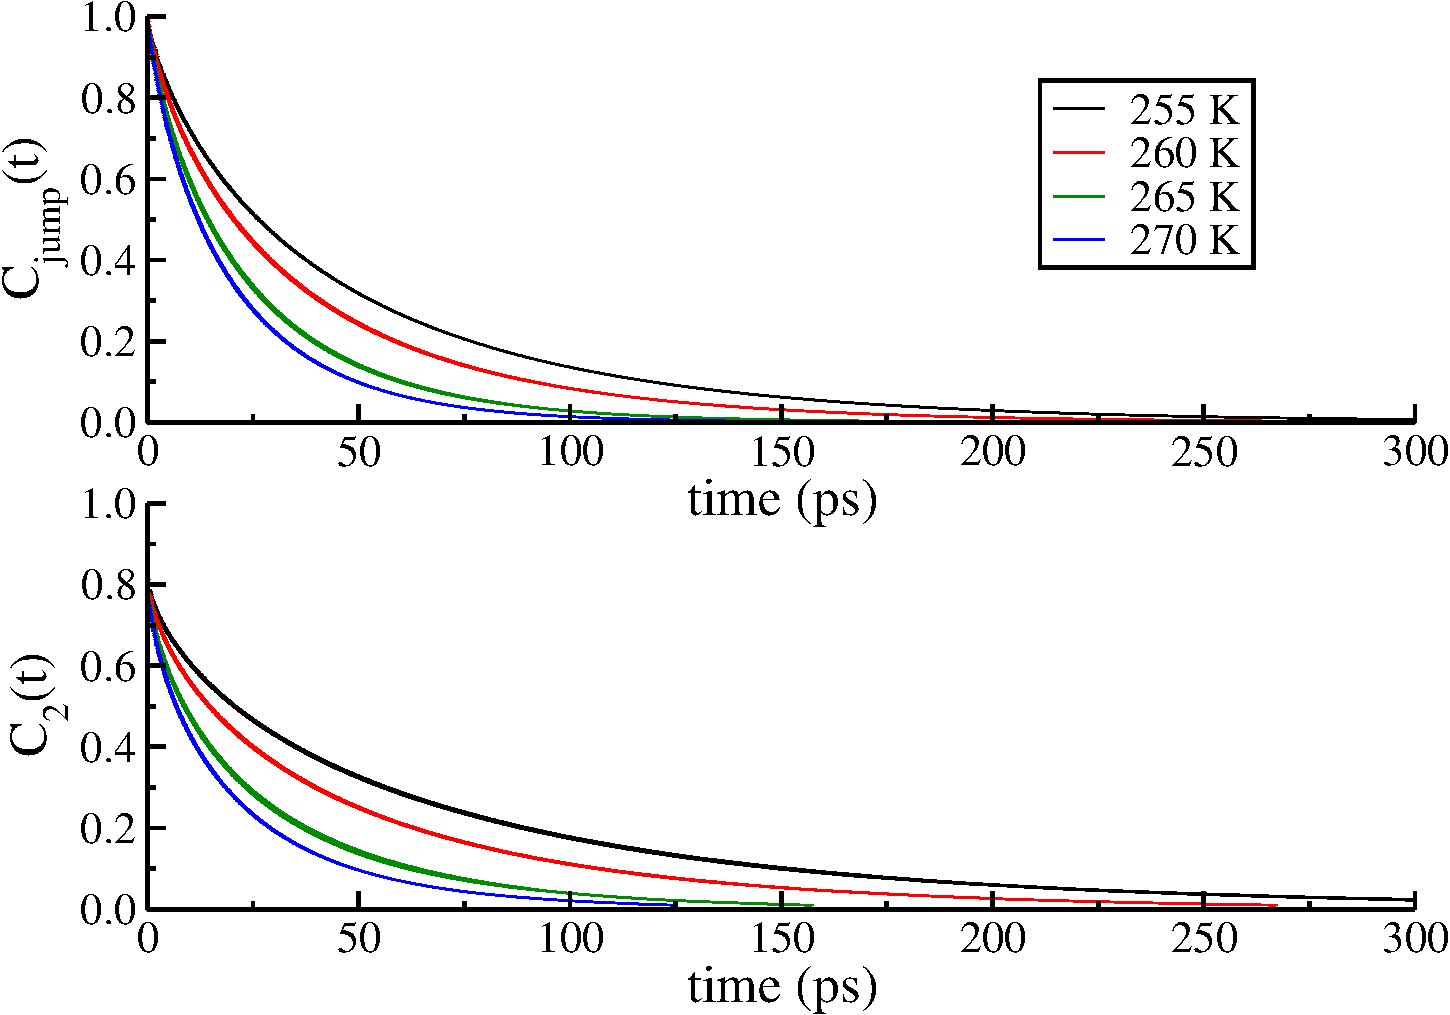
\includegraphics[width=\linewidth]{Figures/jump_lcorr}
\caption{\label{fig:jump_lcorr} The orientational time correlation
  function C$_2$(t) (lower panel) and the hydrogen bond jump
  correlation function C$_\mathrm{jump}$(t) (upper panel) for
  supercooled liquid water. }
\end{figure*}                


\begin{flushleft}
\textit{Hydrogen Bond Jump Times}
\end{flushleft}
The hydrogen bond jump time measures the decorrelation of a hydrogen
bond between two water molecules, $a$ and $b$. 
\begin{equation}\label{jump}
C_\mathrm{jump}(t) = 1 - \langle n_a(0) n_b(t) \rangle
\end{equation}
$n_a(0)$ is set to 1 if hydrogen $i$ is bound to water molecule $b$ at
time ($t=0$), and set to zero otherwise. A spatially resolved version
of this correlation function was described in Chapter \ref{chap:Dyn},
while here we are interested in the temperature dependence of the
hydrogen bond jump times. Again absorbing boundary conditions were
applied, \textit{i.e.} any back jumps were considered new hydrogen
bonds forming.

The hydrogen bond jump correlation function was computed for each of
the bulk liquid simulations, and the resulting $C_\mathrm{jump}(t)$
are plotted in the upper panel of Figure \ref{fig:jump_lcorr}. These
were found to be well fit by a single exponential decay, with a decay
constant describing the jump time for breaking and making hydrogen
bonds. From these characteristic decay times the jump rate can be
determined $k_\mathrm{jump} = \tau_\mathrm{jump}^{-1}$. These jump
rates are presented in Table \ref{tab:bulkJump}. We observe a clear
temperature dependence in the jump rates, at colder temperatures the
jump rates are smaller, around $k_\mathrm{jump} = 0.016$ (ps$^{-1}$),
and at warmer temperatures $k_\mathrm{jump} = 0.04$ (ps$^{-1}$).

\begin{table}[h] \centering \caption{HYDROGEN BOND JUMP RATES FOR THE
    SUPERCOOLED BULK LIQUID\label{tab:bulkJump}}
\begin{tabular}{cc}
\hline
\hline
 Temperature & $k_\mathrm{jump}$ \\
\hline
270 & 0.0402(7) \\
265 & 0.0328(7) \\
260 & 0.0207(3)  \\
255 & 0.0160(5) \\
\hline
\hline
\end{tabular}
\begin{flushleft}
  Temperatures are given in K, and jump rates are presented in
  ~ps$^{-1}$. Uncertainties are given in parentheses.
\end{flushleft}
\end{table}

           

\subsection{Shear Viscosity of Supercooled Liquid}
In order to compare the shear viscosities of the quasi-liquid layers,
velocity shearing and scaling reverse non-equilibrium molecular
dynamics simulations were performed on a bulk supercooled liquid. A
liquid box containing $16,000$ TIP4P/Ice water molecules with
dimensions $\mathrm{L_x} = 51.22~\mathrm{\AA}$,
$\mathrm{L_y} = 51.22~\mathrm{\AA}$, and
$\mathrm{L_z}=200.87~\mathrm{\AA}$ was subjected to a simultaneous
kinetic energy and momentum flux. This resulted in simultaneous
thermal and velocity gradients across the $z$ dimension of the
simulation box. The velocity profile was fit with a quadratic
regression, and an analytic derivative with respect to the $z$ gave
$(\frac{\partial V_x}{\partial z}$). Together with the imposed
momentum flux gives the shear viscosity.
\begin{equation}\label{eq:viscosity}
  j_{z}(p_{x}) = -\eta \big(\frac{\partial v_{x}}{\partial z}\big)
\end{equation}
The temperature gradient through the system was fit with a linear
regression. Using this regression, the local temperature for each
$\eta$ was obtained.  

The resulting $\eta$ values were fit with the Williams-Landel Ferry model (WLF)
for predicting the shear viscosity of polymers and other liquids which
exhibit a glass transition temperature ($T_g~\sim~136~\mathrm{K}$ for
water). 
\begin{equation}\label{eq:WLF}
\eta (T) = \eta_0 \exp \Bigg({\frac{-C_1 (T-T_r)}{C_2 + T - T_r}}\Bigg)
\end{equation}
Here, $\eta_0$, $C_1$, $C_2$, and $T_r$ are empirical
parameters. Typically, $T_r$ is taken to be the glass transition
temperature ($T_g$), and when this choice is made $C_1$ and $C_2$ are
characteristic of the class of material being
fit. With this it is possible to estimate the temperature dependence
of the shear viscosity by knowing it only at one data point. Our data
and resulting fit can be seen in Figure \ref{fig:etaT}.
\begin{figure*}
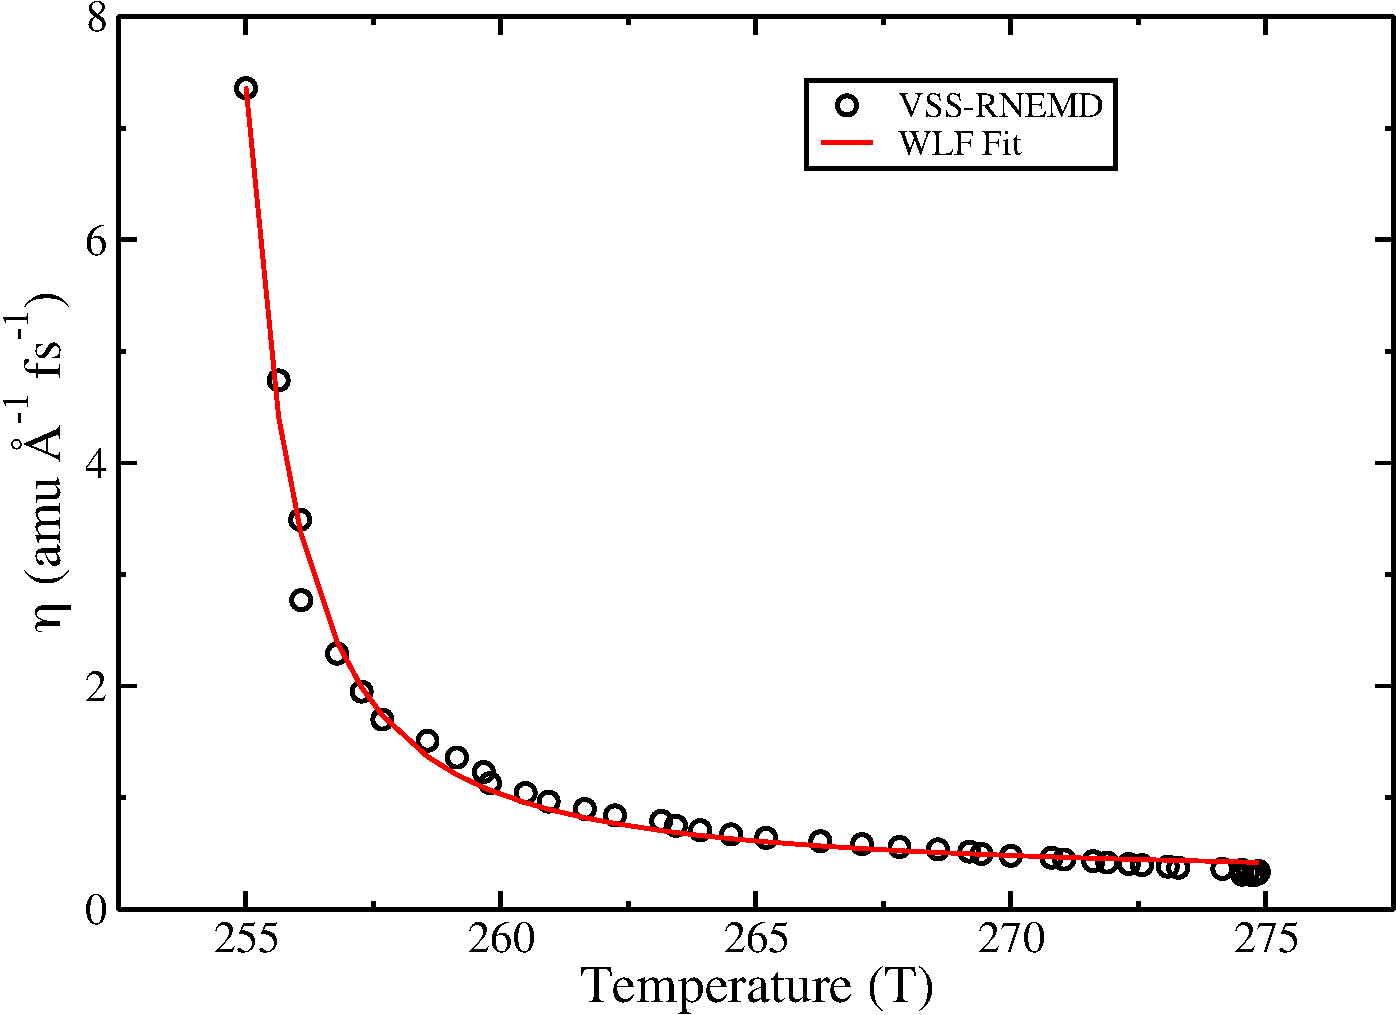
\includegraphics[width=\linewidth]{Figures/etaT}
\caption{\label{fig:etaT} The shear viscosity $\eta$ of supercooled
  liquid water as a function of temperature. The black circles are
  data computed from a single VSS-RNEMD simulation with simultaneous
  kinetic energy and momentum fluxes, the red curve is a fit described
  by the Williams-Landel Ferry model.}
\end{figure*} 
Querying the fit at the four temperatures the ice surfaces were
investigated at, we can obtain reasonable estimates of the shear
viscosity for the supercooled bulk liquid. These values are reported
in Table \ref{tab:bulkVisco}.
   

\begin{table}[h] \centering \caption{SHEAR VISCOSITY OF THE
    SUPERCOOLED BULK LIQUID\label{tab:bulkVisco}}
\begin{tabular}{cc}
\hline
\hline
 Temperature & $\eta$ \\
\hline
270 & 0.5 \\
265 & 0.6 \\
260 & 1.0  \\
255 & 7.3 \\
\hline
\hline
\end{tabular}
\begin{flushleft}
  Temperatures are given in K, and shear viscosities are reported in
  (amu~\AA$^{-1}$~fs$^{-1}$).
\end{flushleft}
\end{table}


\section{Discussion}
Conde \textit{et al.} investigated water model dependence on the
formation of the quasi-liquid layer at the vapor exposed basal,
prismatic, and secondary prismatic surfaces of
ice-I$_\mathrm{h}$.\cite{Conde2008} They established a cutoff value in
the local tetrahedral order parameter, $q_t$, to denote molecules as
being ice-like or liquid-like. Using this, they estimated QLL widths
to be $\sim$~5-10~\AA~ for the TIP4P/Ice model over the range of
temperatures investigated here. 

In order to compare with Conde
\textit{et al.}, we have fit the tetrahedrality profiles with a
hyperbolic tangent which is designed to transition smoothly between
the vapor / QLL / ice interfaces.
\begin{equation}\label{eq:qllFit}
q(y) \approx
q_\mathrm{vap}+\frac{q_\mathrm{ice}-q_\mathrm{qll}}{2}\left[\tanh\left(\frac{y-l}{w^q}\right)-\tanh\left(\frac{y-u}{w^q}\right)\right]
\end{equation}
Here, $q_\mathrm{vap}$ and $q_\mathrm{ice}$ are are the values for $q$
in the vapor and ice, $l$ and $u$ are the lower and upper interfaces,
and $w^q$ is the width of that interface, that is, the width of the
quasi-liquid layer.  We estimate the vapor / ice-I$_\mathrm{h}$
interface to be approximately 7-12~\AA~wide for both the basal and
prismatic surfaces at each of the temperatures investigated. While
slightly larger, these values agree well with the estimates of Conde
\textit{et al.}. 

As described in Chapter \ref{chap:Methods}, the basal and prismatic
surfaces used in this study exhibit proton ordering at the surface of
the crystal. This was chosen to reproduce observed ordering at the
surface of ice, although the ice surface used by Conde \textit{et al.}
presents disordered protons. Our results here indicate that the
proton-ordering at the basal and prismatic surfaces of
ice-I$_\mathrm{h}$ do not significantly alter the width of the QLL as
compared to proton disordered surfaces.  Furthermore, Conde
established that the SPC/E, TIP4P, TIP4P/2005, and TIP4P/Ice models
estimated QLLs of similar thickness, when compared to the relative
undercooling temperature of the model.\cite{Conde2008} Given that our
estimates of the thickness of the QLL agrees with that of Conde, we
believe our estimates should be robust for other water models as well,
but we have no evidence of this.

Neshyba \textit{et al.} investigated sublimation and deposition of
water molecules at the ice / vapor interface.\cite{Neshyba2009} They
also observed the formation of a QLL while using the NE6
model\cite{Nada2003a} at 250 K (T$_\mathrm{m}$ - 48 K for the NE6
model), and discriminated the QLL molecules by their intermolecular
potential energy. Doing so, they designated two separate QLLs, which
we have described as a single QLL here. They distinguish an outer QLL
which contains roughly 8\% of the total molecules, and an inner, more
crystalline QLL containing the remaining 92\%. 

In addition to obtaining estimates of the QLL width, Equation
\eqref{eq:qllFit} provides locations of the QLL which can be used to
query other properties, such as the diffusion coefficient or shear
viscosity. For the basal surfaces, $l$ and $u$ are found to be
approximately $\pm$~20.5 ~\AA~ from the center of the ice. Similarly,
the prismatic interfaces are found to be $\sim~\pm$~23.5~\AA~ from the
center of the ice, respectively. For both surfaces, there is no
temperature dependence on the locations of $l$ and
$u$. Therefore, we will use these locations for querying additional
structural and dynamic properties to establish characteristics of the
surface premelt. The average value of the tetrahedrality, diffusion
constant, and shear viscosity for the two interfaces at each
temperature is reported in Table \ref{tab:qllResults}.

\begin{table}[h] \centering \caption{STRUCTURAL AND DYNAMIC
    PROPERTIES OF THE QUASI-LIQUID LAYER\label{tab:qllResults}}
\begin{tabular}{rcccc}
\hline
\hline
Surface & Temperature & $q$ & D & $\eta$ \\
\hline
\multirow{ 4}{*}{Basal  $\{0001\}$} & 270 & 0.744(2) &2.3(7) & 0.17(5)\\ &265 &
                                                                    0.748(1)&
                                                                              1.8(2) & 0.20(1) \\ &260 &  0.759(4)& 1.10(1) & 0.33(1) \\ &255 & 0.764(2) & 0.80(4) & 0.46(2) \\
\hline
\multirow{ 4}{*}{Prismatic  $\{10\bar{1}0\}$} & 270 & 0.856(1) &  1.3(2) &  0.30(1) 
\\ & 265 & 0.867(2) &0.8(4) & 0.5(3) \\ & 260 & 0.879(1) & 0.5(3) &
                                                                      0.8(3) \\
        & 255 & 0.887(2) &0.34(3) &0.96(6)\\
\hline
\hline
\end{tabular}
\begin{flushleft}
  Temperatures are given in K, diffusion constants in
  (x$10^{-5}$~\AA$^{2}$~fs$^{-1}$),~ and shear viscosities in
  (amu~\AA$^{-1}$~fs$^{-1}$).
\end{flushleft}
\end{table}

From Table \ref{tab:qllResults}, we see a clear temperature dependence
in all three properties reported for the basal interface. The local
tetrahedral order parameter increases with decreasing temperature,
indicating a more structured environment. The diffusion constant
decreases with decreasing temperature, and as expected from Equation
\eqref{eq:stokes-einst}, this results in an increase in the shear
viscosity.  The results for the prismatic interface follow the same
trend. With decreasing temperatures, the local structure of the QLL
becomes more tetrahedral, and diffusion within the QLL is reduced. 

It is interesting that the value for the tetrahedrality for the QLL is
different for the basal and prismatic surface, as this was not true
for the Gibbs dividing surface at the ice / bulk liquid simulations
described in Chapter \ref{chap:Str}. The prismatic QLL has a slightly
larger $q$~value than that of the basal, values of $q~\sim~0.85$ as
compared to $q~\sim~0.75$.  This may be a result of the basal interface
having a more diffuse vapor phase, or that perturbations made by the
presence of the surface extends further into the ice crystal for the
basal facet than the prismatic.

The diffusion constants for the two surface premelts are significantly
different. At the basal face, values of
$\mathrm{D}~\sim~2.3$~(\AA$^{2}$~fs$^{-1}$) to
$\mathrm{D}~\sim~0.8$~(\AA$^{2}$~fs$^{-1}$) are observed. This is
significantly larger than those at the prismatic surface,
$\mathrm{D}~\sim~1.3$~(\AA$^{2}$~fs$^{-1}$) to
$\mathrm{D}~\sim~0.3$~(\AA$^{2}$~fs$^{-1}$). At each temperature
investigated, D$_\mathrm{prismatic} \approx 2$
D$_\mathrm{basal}$. This trend agrees well with the coefficients of
friction ($\kappa$) at the ice / water interface reported in Chapter
\ref{chap:Friction}, where we found
$\kappa_\mathrm{prismatic} \approx 2 \kappa_\mathrm{basal}$. These
results indicate diffusion on the basal surface is faster than
compared to the prismatic, which was observed to have a larger
friction coefficient. Given this, it is not surprising that the shear
viscosities of the QLL at the basal surface are smaller than those
found at the prismatic surface.

Pfalzgraff \textit{et al.}\cite{Pfalzgraff2011} and later Gladich
\textit{et al.}\cite{Gladich2011,Gladich2015} observed anisotropic
diffusion of the QLL on the prismatic, 14\degree~ pyramidal, and
secondary prismatic surfaces of an ice-I$_\mathrm{h}$ crystal. This
behavior was prominent at colder temperatures where the QLLs were thin
and the water contributing to the QLL is significantly influenced by the
underlying crystal structure. At warmer temperatures and
correspondingly thicker QLLs, isotropic diffusion is recovered. While
one dimensional diffusion coefficients were not resolved here, their
results may suggest that the shear viscosity of the QLLs is
directionally dependent at colder temperatures. 

Comparing the shear viscosities of the QLL with the values obtained
for supercooled liquid water in Table \ref{tab:bulkVisco}, we see that
the bulk liquid agrees within error of the prismatic QLL at 265 K and
260 K. Below 260 K, the shear viscosity of the bulk liquid diverges as
it approaches its glass transition temperature. Due to this, the bulk
shear viscosity at 255 K is much larger than predicted for any of the
QLLs studied here. Also, at all temperatures investigated the shear
viscosity of the basal QLL is significantly smaller than computed for
the bulk liquid. 

There are a few reasons why we see disagreement between the
supercooled liquid and the QLL viscosities. The smaller values of
$\eta$ obtained for the surface premelt may be due to the open vapor
phase. In contrast, the bulk liquid at the same temperature is
subjected to a more confined space. Molecules in the QLL can move
through the diffuse vapor, resulting in larger mean squared
displacements. Similarly, molecules in the QLL may be able to more
easily move tangentially through the QLL due to the open interface, as
the resistance to motion is reduced due to the low density of
molecules.

A second possibility is that the local structure of the molecules
in the QLL is different from that of the bulk liquid. From the top
panel of Figure \ref{fig:gofrQ}, the supercooled bulk liquid's
tetrahedrality distribution has a maximum of about $q \sim$~0.89, and
is observed to decrease slightly with increasing temperature. However,
even for bulk liquid at 270 K, the distribution is centered around
$q \sim$~0.86, which is in agreement with our estimates of $q$ at the
prismatic surface ($q~\sim~0.85$). The bulk liquid has a rather broad
distribution in $\rho (q)$, however, and the observed differential
viscosities could stem from low population regions of this
distributions. 

It would be interesting to resolve beyond error the spatial dependence
of the shear viscosity for both of the QLLs, as surface premelt closer
to the ice (in a more confined environment) may behave more like
the supercooled bulk liquid. Also, the surface might impose significant
drag on the QLL at short distances normal to the surface. In addition,
computing the fractional densities of tetrahedral ordering at the
surfaces of ice may illuminate more on the observed discrepancies
between the bulk and QLL viscosities. 



% Similarly, Dehaoui
% \textit{et al.} have measured the viscosity of supercooled water down
% to -34\degree C without freezing the liquid.\cite{Dehaoui2015} There
% have been suggestions that Equation \eqref{eq:stokes-einst} breaks
% down at temperatures close to T$_\mathrm{g}$, the glass transition
% temperature, implying that the translational diffusion and the shear
% viscosity of the liquid become decoupled.


% As seen in Figure \ref{fig:qll-rhoq}, the QLLs at the surface of the
% basal and prismatic crystals form a bilayer. Following Neshyba
% \textit{et al.}, we denote the following definitions; molecules within
% the ice are labeled as $\mu_{i}$, where each $i$ denotes a unique
% density peak in the ice, molecules in the QLL layer closer to the ice
% are labeled as $\epsilon_{2}$, and molecules in the outer portion of
% the QLL bilayer are labeled as $\epsilon_{1}$.\cite{Neshyba2009} Due
% to their relative distances from the underlying crystal, molecules
% within layers $\epsilon_{2}$ and $\epsilon_{1}$ experience vastly
% different local environments. Water molecules within $\epsilon_{2}$
% located closer to the ice experience significantly more drag than
% those closer to the vapor. Therefore, we expect a noticeably different
% sheer viscosity for the molecules located in $\epsilon_{2}$ and
% $\epsilon_{1}$. 


% % In a recent review of Ice Surfaces, Mary Jane Shultz posed numerous
% % open questions about the qll, such as what is the growth mechanism,
% % relative energies of various faces are not well understood, what is
% % the impact of face termination on ice surface energy and reactivity,
% % what defintion is relevant for the qll, at what temperature does the
% % qll from, what is the nature of the qll?

% 2017 PNAS paper by M. Alejandra Sanchez \textit{et al.} provides
% experimental (surface-specific vibrational sum frequency generation
% spectroscopy)  and theoretical (molecular dynamics simulations with
% the TIP4P/Ice model)
% evidence that the qll formation occurs
% bilayer-by-bilayer. Observed for the basal face and the secondary prism. 

% % Determination of Surface Tension-to-Shear Viscosity Ratio for
% % Quasi-liquid layers on Ice Crystal Surfaces.
% %   K. Murata, H. Asakawa, K. Nagashima, Y. Furukawa, G. Sazaki
% %   PRL 115 (2015) 256103
% Using laser confocal microscopy in conjunction with an inverted
% optical microscope, Murata \textit{et al.} have recently measured the
% characteristic-velocity (\textit{i.e.} the surface tension-to-shear
% viscosity ratio) of two distinct wetting morphologies of QLLs on the
% basal surface of ice at -0.2 degrees Celcius and a pressure of 578.9
% Pa.\cite{Murata2015} They observed a partial wetting QLL, described as
% a bulk liquid droplet (BLD), as well as a complete wetting state,
% described as a thin liquid layer (TLL). The characterstic-velocity of
% the BLDs was determined from relaxation modes of their contact lines,
% which was observed to decay with single exponential behavior according
% to
% \begin{equation}
% u_q = u_q(0) exp\Bigg(-\frac{V^* \theta^3 q}{3l}t\Bigg)
% \end{equation}
% where $q$ is the wave vector for the perturbing mode for the
% relaxation of the amplitude of the contact line and $u_q(0)$ being the
% initial amplitude of the mode. Here, $V^* = \gamma / \eta$ is the
% characteristic velocity and $\theta$ is the contact angle the BLD makes
% with the ice surface ($\sim$ 2 degrees). Lastly, the logarithmic factor
% $l=ln(L/a)$ is a cutoff parameter which helps avoid
% singularities. From this fit, they obtained $V^* = 2 \pm 1$ m/s, which
% is about an order of magnitude smaller than that of bulk water, 42.21
% m/s.

% Murata \textit{et al.} also investigated the spreading dynamics of the
% BLD-QLLs, during the transformations to TLL-QLLs. The radii of the
% spreading BLD-QLLs were fit to a power law
% \begin{equation}
% r = L (\frac{4S}{3Ll \eta})^{1/4}(t+t_0)^{1/4}.
% \end{equation}
% Here, $S$ is the spreading coefficient, and $t_0$ captures the initial
% state of the droplet. As the QLL transitions from the BLD
% drpolet-shape to the TLL pancake-shape, the volume must be
% conserved. From this conservation, Murata \textit{et al.} estimated
% the thickness of the TLLs as 9 $\pm$ 3 nm.

% Lastly, Murata \textit{et al.} have obtained the characteristic
% velocity of the TLLs in the same way as the BLDs. However, here the
% hydrodynamic dissipation is not located at the wedge of the droplet
% like in the BLD case, but instead the dissipation occurs within the
% fluid of the pancake-shape object itself. Due to this, a slightly
% different expression for the viscous force must be used, and the
% resulting characteristic velocity was found to be $V^* = 0.2 \pm 0.1$
% m/s, about 200 times smaller than that of bulk water. This seems to
% imply a dependence on the characteristic velocity to the QLLs contact
% area and distance from the surface. The BLD droplet-shaped QLLs (where
% the QLL is only partially wets the surface and a larger amount of the
% QLL resides further from the surface), were found to have a
% characteristic velocity of about an order of magnitude larger than the
% more completely wetting state, where more of the QLL resides closer to
% the surface.

% It is interesting to note that the surface tension of the BLD/air
% interface ($\gamma_t$) is approximately equal to the TLL/air interface
% surface tension ($\gamma_b$), as there is observed coexistence of both
% forms of QLLs at the same time. Therefore, the discrepancy in $V^*$
% can be primarily attributed to the shear viscosity of the QLL phase.
 
% % end Murata2015


% Discuss widths of qll by experimental groups. Probing different
% measures of the qll gives different widths at different
% temperatures. Give a quick summary of the kinds of experiments and
% what their findings were for qll widths.




% Break down of stoke's-einstein relation for viscosity. \cite{Chen2006,
%   Tarjus1995,Bordat2003,Kumar2007}


% % The thickness of a liquid layer on the free surface of ice as
% % obtained from computer simulation. M.M.Conde, C.Vega, A.Patrykiejew
% % JCP 129, 014702 (2008)
% %Outstanding references and background
% Molecular dynamics simulations of ice-I$_\mathrm{h}$ with a free
% surface were performed using the SPC/E, TIP4P, TIP4P/Ice, and
% TIP5P/2005 water models. The basal, prismatic, and secondary prismatic
% surfaces exposed to vacuum were analyzed. Conde \textit{et al.}
% observed that the thickness of the liquid like layer that develops on
% the surface of the ice is of approximate thickness for a given plane
% across all water models, when comparison is made at the same relative
% undercooling temperature for the water models.\cite{Conde2008} In all
% cases the width of the liquid layer is found to increase with
% increasing temperature. For a given temperature, the following trend
% in QLL thickness was observed, the basal plane > the primary prismatic
% plane > the secondary prismatic plane. For the TIP4P/Ice model, the
% onset temperature of the QLL was observed at -100 degrees Celcius for
% the basal plan, -80 degrees Celcius for the primary prismatic plane,
% and -70 degrees Celcius for the secondary prismatic plane. NVT
% simulations between 6 and 12 ns. To discriminate icelike and
% liquid-like water molecules, they have used the local tetrahedral order
% parameter of Errington and Debenedetti. However, their values are
% locked at only the four closest neighbors.

% Conde \textit{et al.} have computed probability densities of the local
% tetrahedral order parameter, $p(q)$, for both a bulk liquid and bulk
% icesystem for all the models investigated. The TIP4P model results
% were almost indistinguishable, and the SPC/E model results were in
% good agreement with the TIP4P/Ice results considering the large
% discrepancy between the melting points of the models. However, there
% is visible overlap between the bulk liquid and bulk ice distributions,
% making discrimination between icelike and liquid-like molecules
% difficult. Therefore, they defined a cutoff value of $q$, denoted
% $q_{t}$, where molecules with $q < q_t$ are denoted to be liquid-like,
% and molecules found with $q > q_t$ are denoted as ice-like. 
% \begin{equation}
% \int_{q_t}^{1} p_{liquid}(q)dq = \int_{0}^{q_t} p_{I_h}(q)dq
% \end{equation}
% Here, $\int_{q_t}^{1} p_{liquid}(q)dq$ is the probability of
% incorrectly assigning a liquid-like water molecule as icelike, and
% similarly $\int_{0}^{q_t} p_{I_h}(q)dq$ is the probability of
% incorrectly assigning an icelike water molecule as
% liquid-like. Graphically, $q_t$ is the value of $q$ where the area
% under the $p_{liquid}(q)$ curve to the left of $q_t$ is equal to the
% area under the $p_{I_h}(q)$ curve to the right of $q_t$.  The values
% for $q_t$ were found to be approximately the same for each model
% investigated, with $q_t$ (SPC/E) $\sim 0.9101$ and
% $q_t$ (TIP4P/Ice) $\sim 0.9076$. 

% The width of the QLL was obtained by
% \begin{equation}
% \delta =
% \frac{N_\mathrm{liquid}M}{2\rho N_\mathrm{AV}L_\mathrm{y}L_\mathrm{z}}
% \end{equation}
% where $N_{liquid}$ is taken to be the average number of liquid-like
% molecules during the simulation, $M$ is the molecular weight of water,
% $N_{AV}$ is Avogadro's number, the product $L_yL_z$ is the area of the
% exposed crystal face, and $\rho$ is the density of liquid water. The
% factor of 2 in the denominator accounts for the two interfaces which
% are presented by the crystal in the simulation cell. However, their
% definition of the thickness of the QLL is inherently flawed in the
% following way. Since their definition of liquid-like molecules comes
% from their local tetrahedral order number which assumes four nearest
% neighbors, molecules at the surface of the crystal will have an
% artificially low value for $q$ and be labeled as liquid-like, even
% though their structure (based on angles between neighbors) is
% indicative of an icelike environment. A rescaling based on the number
% of neighbors present would give a more accurate result. 

% Conde \textit{et al.} also considered a dynamic criteria for whether a
% water molecule is liquid-like or icelike. They computed the mean-square
% displacement of each water molecule, and compared these values to
% reference data of the TIP4P/2005 water model mean-square displacement
% of bulk ice and bulk liquid water simulations. They quantified an
% icelike molecule to have a mean-square displacement of less than 1
% \AA~ after 400ps, and classified molecules as liquid-like if their
% mean-square displacement was greater than 1 \AA~ otherwise. While the
% structural and dynamic widths are not precisely the same, they are on
% the same order of magnitude, similar to our own results. 
% %end Conde2008


% %Anisotropy in structural phase transitions at ice surfaces: a
% %molecular dynamics study. H. Nada and Y. Furukawa, 1997, Applied
% %Surface Science, 121/122, 445-447. Nada1997
% 720 water molecules in each ice slab, exposing the basal and prismatic
% surfaces. basal system was (22.4 x 23.3 x 43.8) \AA and the prismatic
% system was (22.4 x 21.9 x 46.6) \AA. The TIP4P water model was
% used. Simulations were performed between temperatures of 220 and 250
% K, in incrementes of 5 K. NVT simulations performed. To estimate the
% thickness of the quasi-liquid layer, root mean square fluctuations in
% the oxygen-oxygen length between molecules was calculated for bins of
% molecules normal to the interface.
% \begin{equation}\label{eqNada1997-1}
% \delta = \frac{2}{n(n-1)} \sum_{i<j}^{n}
% \frac{\sqrt{<r_{ij}^{2}>-<r_{ij}>^{2}}}{<r_{ij}>}
% \end{equation}
% Here, $n$ denotes the number of water molecules, $r_{ij}$ the distance
% between oxygen atoms of water molecules $i$ and $j$ respectively, and
% the angle brackets denote a times average. For a slice of molecules
% with a $\delta \ge 0.1$, they are denoted as satisfying the criteria
% to be a quasi liquid layer. This criteria is known as the Linemann
% criterion (ref. 11 therein). Nada and Furukawa estimated the width of
% the QLL to be about 11.5 \AA for the basal ice/vapor interface, and 9
% \AA for the prismatic interface, respectively. They also observe
% increasing QLL thickness with increasing temperature. Also, for low
% temperatures, they observed the prismatic surface having a thicker
% QLL, while at higher temperatures, the basal QLL was predicted to be
% thicker, with the transition occurring around 235~K. \cite{Nada1997}
% %end Nada1997

% % Anisotropic Surface Melting of an Ice Crystal and its Relationship
% % to Growth Forms. Y. Furukawa and H. Nada. J. Phys. Chem. B 1997,
% % 101, 6167-6170.
% Experiments have shown that anisotropic surface melting occurs on the
% surface of the basal and prismatic faces of an ice crystal, just below
% the melting point. That is, at temperatures approaching the melting
% point, the basal QLL is thicker than the prismatic QLL. 

% A nice summary of ellipsometry measurements is given in the
% intro. References 12 and 14 therein, simultaneously measured both the
% thickness of the QLL as well as the index of refraction of the
% transition layer on the ice surface using null ellipsometry (what is
% null ellipsometry). From -2 degrees Celcius, the thickness of the QLL
% steeply increased with increasing temperature. The index of refraction
% was found to be 1.330 (which converts to a density of 991
% $kg/m^{3}$. Comparatively, the index of refraction for water is 1.333
% and bulk ice is 1.308. The QLL thickness of the prismatic facet was
% found to be proportional to $delta T ^{-1/3}$ above -2 degrees
% celcius, while the basal temperature dependence was much steeper. They
% also observed a flat facet at the melting point for the basal face,
% however, the prismatic facet exhibited a rounded surface at -2C. Thus
% a roughening transition is believed to occur on the prismatic facet
% while not on the basal facet.\cite{Furukawa1997} 

% Current work, TIP4P water model for 720 water molecules. At 250~K, the
% basal face has a thinner QLL than the prismatic. This turns over at
% 260~K where they are approximately equal width, and at warmer
% temperatures the basal is observed to have a thicker QLL. Furukawa and
% Nada used the $S$ order parameter of Karim and Haymet which depends on
% the orientational ordering of neighboring molecules.\cite{Karim1988}
% This parameter is unity for an ordered arrangement of water molecules
% in an ice crystal, and $\approx$ 0.3 for a random
% arrangement. Furukawa and Nada defined QLL to be present only if a
% slice of water molecules had $S \le 0.1$. References 18 and 22 therein
% describe the basal/water interface as being smooth, while the
% prismatic/water interface as being diffuse. In addition, reference 22
% shows that the basal facet grows in a layer-by-layer process while the
% prismatic facet grows by a collective incorporation process. 
% %end Furukawa1997


% \subsubsection{Anisotropic Diffusion of the QLL}
% One dimensional diffusion coefficients (D$_\mathrm{i}$) were computed
% via the Einstein's relation\cite{Allen1987}
% \begin{equation}
% D_{i} = \frac{1}{2} \frac{dMSD_{i}(t)}{dt}
% \end{equation}
% where MSD$_\mathrm{i}(t)$ is the mean square displacements as a
% function of time. Gladich \textit{et al.} were careful to exclude any
% sublimating water molecules from being included in their calculation,
% as these molecules move considerably further distances in time than
% their condensed phase counterparts. These MSD$_\mathrm{i}(t)$ were
% staggered in starting time by 20~ps, averaged, and from this average
% MSD$_\mathrm{i}(t)$ the $D_\mathrm{i}$ were obtained by fitting the
% linear portion of the MSD$_\mathrm{i}(t)$ plots, between 5 and 25
% ns. However, they argue the obtained $D_\mathrm{i}$ values need
% correction, as the molecules residing in the solid ice, and ice-like
% molecules within the QLL are incorporated into the calculation of
% $D_\mathrm{i}$ through MSD$_\mathrm{i}(t)$ at this point. They assume
% only liquid-like molecules in the QLL contribute to the surface
% diffusivity, and compute surface diffusion constants
% $D^{*}_\mathrm{i}$ according to\cite{Pfalzgraff2011}
% \begin{equation}\label{D*}
% D^{*}_\mathrm{i} = D_\mathrm{i}/Q
% \end{equation}
% where $Q$ is the mean number of molecules classified as liquid-like
% ($N_\mathrm{LL}$) divided by the total number of molecules in the
% system ($N_\mathrm{Slab}$). They obtain $Q$ by the following simple
% ration, where they exclude sublimating molecules ($N_\mathrm{EV}$
% since they were removed from the MSD$_\mathrm{i}(t)$ calculations
% earlier.
% \begin{equation}
% Q = \frac{N_\mathrm{LL} - N_\mathrm{EV}}{N_\mathrm{Slab} -
%   N_\mathrm{EV}}
% \end{equation}
% This approach to obtaining the scaling parameter $Q$ improves upon the
% method of Pfalzgraff \text{et al.}\cite{Pfalzgraff2011}, where they included every
% molecule in one ice bilayer, including those that had
% sublimated. Using eq. \eqref{D*}, Gladich \textit{et al.} were also
% able to compute two-dimensional surface diffusion constants.
% \begin{equation}
% D^{*}_\mathrm{ij} = (D^{*}_\mathrm{i} + D^{*}_\mathrm{j}) / 2
% \end{equation} 

% Observing the density of the crystal at partitions transverse to the
% interface, Gladich observed the prismatic surface QLL grows
% continuously with increasing temperature. At the lowest temperatures
% investigated, 230~K, only the outermost bilayer was observed to
% participate in the formation of the QLL. At two degrees below the
% melting point of the NE6 model, the density profiles indicated that
% the two outermost bilayers both are involved in the QLL
% formation. This result was similar to those seen by Bishop \textit{et
%   al.}, who studied the basal ice surface also using the NE6 water
% model. These results also agree with those reported by Conde
% \textit{et al.}, who studied QLL on the basal, prismatic, and
% secondary prismatic using the SPC/E, TIP4P, TIP4P/Ice, and TIP4P/2005
% water models.\cite{Conde2008} 

% Gladich \textit{et al.} estimated QLL thickness ($\delta$) relating
% the number of liquid-like quasi-liquid layer molecule
% ($N_\mathrm{LL}$) to the number of water molecules in a bulk liquid
% with box dimensions of $L_\mathrm{x}L_\mathrm{y}\delta$,
% \begin{equation}
% \delta =
% \frac{N_\mathrm{LL}M}{2\rho N_\mathrm{A}L_\mathrm{x}L_\mathrm{y}}
% \end{equation}
% where $M$ is the molar mass of water, $N_{A}$ is Avogadro's number,
% and $\rho$ is the density of liquid water; the factor of two accounts for
% the two interfaces presented by the QLL simulations. Using the
% values of $\rho$ reported by Nada and van der Eerden for supercooled
% liquid water with the NE6 potential,\cite{Nada2003} Gladich computed
% $\delta$ at each temperature investigated, and found the QLL to
% increase from 3.2 \AA~ wide at 59K of undercooling to 7.4 \AA~ at two
% degrees of undercooling.  

% They note a low value of $q$ can be obtained for water molecules
% incorporating an amorphous solid, in which water molecules are four
% coordinate, but are not structured in a tetrahedral arrangement but
% instead in a distorted tetrahedron. 

% Conde \textit{et al.} studied surface QLL on the prismatic facet using
% the TIP4P/Ice water model,\cite{Conde2008} and it was found that the NE6
% model systematically predicts a lower QLL thickness, due to the
% overstructuring of water. Based on their discrimination of
% N$_\mathrm{LL}$ molecules given $q_\mathrm{t}$, the NE6 model was
% found to have a larger value for $q_\mathrm{t}$, which would thus
% result in fewer molecules being considered QLL.

% Gladich \textit{et al.} watched movement of water molecules in the QLL
% along each axis independently, and found at low temperatures that
% movement normal to the interface happened in concert with large
% displacements in the normal plane, even when the normal motion is
% still well within the defined QLL. Therefore, these motions transverse
% to the interface will largely influence surface diffusion of the
% molecules. These motions were in good agreement with the diffusion
% mechanism proposed by Bishop \textit{et al.}\cite{Bishop2009} and by Bolton
% and Pettersson\cite{Bolton2000}, which suggested the outtermost molecules of
% the QLL moved across a relatively rigid surface. Diffusion
% characterized in this way will be highly sensative to the underlying
% surface morphology and topography, mainly, if the surface geometry or
% potential energy surface is anisotropic, we should expect diffusion
% across this surface to also be anisotropic. 

% Observations that in-plane diffusion follows motions transverse to the
% interface were observed at the warmer temperature as well. Through
% this vertical motion, the QLL molecule leaves a well-hydrated local
% environment to the outter portion of the surface where there are fewer
% hydrogen bond partners. Gladich notes that the activation energy for
% diffusion at the warmer temperature might actually be larger than that
% for the colder. With increasing temperature and a thicker
% surface premelting forming, the differing surface topography is masked
% and thus there is no observed anisotropy in surface diffusion.

% Plotting the surface diffusion along the two axis independentally
% ($D^{*}_\mathrm{x}$, $D^{*}_\mathrm{z}$) against inverse temperature,
% the activation energy ($E_\mathrm{a}$) for the diffusion was
% extracted. Since the curvature of ln$D^{*}$ by inverse temperature is
% positive, Gladich concludes the activation energy for the
% high-temperature mechanism for diffusion is greater than that of the
% low-temperature. They further estimate these values to be 29.1 kJ
% mol$^{-1}$ for $E_\mathrm{a}$ the low-temperature (approximately the
% energy of on hydrogen bond with the NE6 model, 24.5 kJ mol$^{mol-1}$) and 24.5 kJ
% mol$^{-1}$ for that of the high-temperature (roughly two hydrogen bonds). 

% Nasello \textit{et al.} investigated surface diffusivity of ice by
% observing the formation of grain boundaries on polycrystalline ice
% surfaces.\cite{Nasello2007} Gladich's computed values for surface diffusivity
% agree well with those by Nasello as Gladich's values fall within the
% error bars reported by Nasello. Gladich's work agrees well with the
% experimental work reported by Price \textit{et al.}\cite{Price1999},
% especially at warmer temperatures. At cooler temperatures however,
% Gladich seems to underestimate surface diffusivity.

% It is interesting to note that at warm temperatures, simulations of
% supercooled bulk liquid\cite{Picaud2006} have also reproduced surface
% diffusivity measured by Price \textit{et al.}. However, the
% supercooled bulk liquid simulations predict a negative Arrhenius
% curvature, implying the activation energy of diffusion decreases with
% increasing temperature, opposite of that observed by Price \textit{et
%   al.} and predicted by Gladich \textit{et al.}. Given the difference
% in sign for the estimated activation energies, it is clear the
% mechanism predicted in each case is drastically different. 

% Gladich \textit{et al.} estimated the temperature at which the
% anisotropic surface diffusivity becomes isotropic by plotting the
% ratio of surface diffusions ($D^{*}_\mathrm{x}$ / $D^{*}_\mathrm{z}$)
% by temperature. They observed a transition to about unity between 240K
% and 250K, between 49 and 39 K of undercooling for the NE6 model.

% % end Gladdich11



% % Arrhenius analysis of anisotropic surface self-diffusion on the
% % prismatic facet of ice. Gladich11, PCCP (2011), 13, 19960-19969
% Using the six-site water model of Nada and van der Eerden (NE6),
% Gladich \textit{et al.} studied surface diffusion of qll water
% molecules on the prismatic surface of an ice-I$_\mathrm{h}$
% crystal.\cite{Gladich2011} Molecules were determined to be part of the
% QLL based on a local tetrahedral order parameter, and only those
% molecules considered QLL were incorporated into the calculations. They
% investigated diffusion over a wide range of temperatures, from 230K to
% 287K, which varies from -59K to -2K of undercooling, when compared
% with the NE6 model's melting point of 289K. The NE6 model overpredicts
% the melting point due to the over structuring of water with the model.

% Their results indicated a positive Arrhenius curvature, suggesting the
% mechanism of self-diffusion changes with increasing temperature. As
% this transition occurs, the energy of activation is also seen to
% increase from 29.1 kJ mol$^{-1}$ at low temperatures to 53.8 kJ
% mol$^{-1}$ at temperatures close to the melting point. The
% self-diffusion is also seen to be anisotropic at low temperatures
% (around XX K), and transitions to isotropic around 240-250K. 

% Using the local tetrahedral order parameter NOT modified for varying
% number of local neighbors. They note that due to this, their estimates
% of 


% \subsubsection{Viscosity of the QLL}


% % Determination of Surface Tension-to-Shear VIscosity Ratio for
% % Quasiliquid layers on Ice Crystal Surfaces.
% %   K. Murata, H. Asakawa, K. Nagashima, Y. Furukawa, G. Sazaki
% %   PRL 115 (2015) 256103
% Using laser confocal microscopy in conjunction with an inverted
% optical microscope, Murata \textit{et al.} have recently measured the
% characteristic-velocity (\textit{i.e.} the surface tension-to-shear
% viscosity ratio) of two distinct wetting morphologies of QLLs on the
% basal surface of ice at -0.2 degrees Celcius and a pressure of 578.9
% Pa.\cite{Murata2015} They observed a partial wetting QLL, described as
% a bulk liquid droplet (BLD), as well as a complete wetting state,
% described as a thin liquid layer (TLL). The characterstic-velocity of
% the BLDs was determined from relaxation modes of their contact lines,
% which was observed to decay with single exponential behavior according
% to
% \begin{equation}
% u_q = u_q(0) exp\Bigg(-\frac{V^* \theta^3 q}{3l}t\Bigg)
% \end{equation}
% where $q$ is the wave vector for the perturbing mode for the
% relaxation of the amplitude of the contact line and $u_q(0)$ being the
% initial amplitude of the mode. Here, $V^* = \gamma / \eta$ is the
% characteristic velocity and $\theta$ is the contact angle the BLD makes
% with the ice surface ($\sim$ 2 degrees). Lastly, the logarithmic factor
% $l=\mathrm{ln}(L/a)$ is a cutoff parameter which helps avoid
% singularities. From this fit, they obtained $V^* = 2 \pm 1$ m/s, which
% is about an order of magnitude smaller than that of bulk water, 42.21
% m/s.

% Murata \textit{et al.} also investigated the spreading dynamics of the
% BLD-QLLs, during the transformations to TLL-QLLs. The radii of the
% spreading BLD-QLLs were fit to a power law
% \begin{equation}
% r = L (\frac{4S}{3Ll \eta})^{1/4}(t+t_0)^{1/4}.
% \end{equation}
% Here, $S$ is the spreading coefficient, and $t_0$ captures the initial
% state of the droplet. As the QLL transitions from the BLD
% drpolet-shape to the TLL pancake-shape, the volume must be
% conserved. From this conservation, Murata \textit{et al.} estimated
% the thickness of the TLLs as 9 $\pm$ 3 nm.

% Lastly, Murata \textit{et al.} have obtained the characterstic
% velocity of the TLLs in the same way as the BLDs. However, here the
% hydrodynamic dissipation is not located at the wedge of the droplet
% like in the BLD case, but instead the dissipation occurs within the
% fluid of the pancake-shape object itself. Due to this, a slightly
% different expression for the viscious force must be used, and the
% resulting characteristic velocity was found to be $V^* = 0.2 \pm 0.1$
% m/s, about 200 times smaller than that of bulk water. This seems to
% imply a dependence on the characterstic velocity to the QLLs contact
% area and distance from the surface. The BLD droplet-shaped QLLs (where
% the QLL is only partially wets the surface and a larger amount of the
% QLL resides further from the surface), were found to have a
% characterstic velocity of about an order of magnitude larger than the
% more completely wetting state, where more of the QLL resides closer to
% the surface.

% It is interesting to note that the surface tension of the BLD/air
% interface ($\gamma_t$) is approximately equal to the TLL/air interface
% surface tension ($\gamma_b$), as there is observed coexistence of both
% forms of QLLs at the same time. Therefore, the discrepency in $V^*$
% can be primarily attributed to the shear viscosity of the QLL phase.
% % end Murata2015

\section{Summary}
In this chapter we have presented simulations of the basal and
prismatic vapor exposed facets of an ice-I$_\mathrm{h}$
crystal. Simulations were performed at four temperatures of
undercooling, and a quasi-liquid layer (QLL) was observed to form at
each of the investigated temperatures. These QLLs were estimated to be
$\sim $~7-12 \AA wide by structural measures, in good agreement with
previous work by Conde \textit{et al.}.\cite{Conde2008} Spatially
resolved three dimensional diffusion coefficients were computed, and
estimates of the shear viscosity were obtained. We observe roughly a
factor of two difference between the diffusion coefficients at the
basal surface as compared to the prismatic, and correspondingly
smaller estimates of the shear viscosity. This trend is in agreement
with the friction coefficients reported in Chapter
\ref{chap:Friction}, where the prismatic facet was observed to be
approximately a factor of two larger.

Simulations of supercooled bulk liquid were performed to compare
against the characteristics of the QLLs. Structural measurements of
the supercooled liquid indicate similar local ordering as compared to
the ice surfaces. At some of the temperatures, the shear viscosity of
the supercooled bulk liquid agrees within error with values computed
for the prismatic QLL. However, $\eta$ for the bulk is observed to
always be significantly larger than the viscosity of the basal QLL. We
attribute the smaller values of $\eta$ for the QLLs to be due to the
presence of the vapor phase, as compared to the volumetrically
constrained bulk liquid. 
